\documentclass[conference]{IEEEtran}
\usepackage{cite}
\usepackage{graphicx}
\usepackage{algpseudocode}
\usepackage{algorithm}

\graphicspath{ {./gambar/} }

\renewcommand\IEEEkeywordsname{Keywords}
%Judul
\title{Implementasi Algoritma Dijkstra Dalam
Menemukan Jarak Terdekat Dari Lokasi Pengguna
Ke Tanaman Yang Di Tuju}

%Penulis
\author{\IEEEauthorblockN{Muhammad Hanif Hibatullah}
\IEEEauthorblockA{\textit{School of Electrical Engineering and Informatics}\\
\textit{Institut Teknologi Bandung}\\
Bandung, Indonesia\\
13220051@std.stei.itb.ac.id
}
}
\begin{document}

\maketitle

\begin{abstract}
    Kebun Raya Purwodadi dengan luas area sekitar 85
    hektar ternyata kekurangan papan informasi yang menyebabkan
    pengunjung kerap kali kebingungan dalam mencari lokasi tana-
    man tertentu. Paper ini bertujuan untuk membuat simulasi
    dari algoritma yang dapat menentukan jarak terdekat antara
    pengunjung (pengguna program) dengan lokasi tanaman yang
    dituju. Algoritma yang digunakan adalah algoritma Dijkstra
    yang beroperasi secara menyeluruh (\textit{greedy}) untuk menguji
    seitap persimpangan (\textit{Vertex}) dan jalan (\textit{Edge}) pada Kebun
    Raya Purwodadi. Berdasarkan hasil simulasi dan pengujian,
    kompleksitas ruang dari program ini adalah O(V) karena adanya
    pembentukan array yang berisi V \textit{nodes} untuk mencari \textit{heap} min-
    imum. Sementara, kompleksitas waktu dari algoritma tersebut adalah \boldmath$O(V^2)$.
\end{abstract}


\begin{IEEEkeywords}
    Dijkstra, \textit{Vertex}, \textit{Edge}, Tanaman.
\end{IEEEkeywords}
\section{Introduction}
    Studi mengenai penggunaan algoritma Dijkstra dalam men-
    cari jarak terdekat dapat diimplementasikan pada kasus pen-
    carian tanaman pada Kebun Raya Purwodadi seperti yang telah
    dilakukan oleh Yusuf et al di tahun 2017~\cite{yusuf2017implementasi}. 
    Paper ini bertujuan untuk melakukan simulasi kembali terhadap penelitian
    yang telah dilakukan dengan bahasa C serta mengevaluasi
    efisiensinya melalui perhitungan kompleksitas waktu dan ru-
    ang dengan analisis Big-O.

    Di Kecamatan Purwodadi, Kabupaten Pasuruan, terdapat
    salah satu kebun raya di Indonesia yang bernama Kebun
    Raya Purwodadi yang memiliki luas area hingga 85 hektar.
    Kebun raya sebagai fasilitas rekreasi dan penelitian ini ternyata
    kekurangan papan informasi yang seharusnya disediakan oleh
    pihak pengelola. Hal ini menyebabkan banyaknya pengunjung
    yang merasa kebingungan untuk mencari lokasi dari tanaman
    tertentu. Oleh karena itu, Yusuf et al (2017) memutuskan
    untuk membuat suatu aplikasi dengan memanfaatkan algoritma
    Dijkstra untuk membantu pengunjung Kebun Raya Purwodadi
    dalam mencari lokasi tertentu.

    Algoritma Dijkstra digunakan karena algoritma ini dapat
    beroperasi secara menyeluruh (algoritma \textit{greedy}) terhadap
    semua alternatif fungsi serta durasi eksekusi yang lebih cepat
    jika dibandingkan dengan algoritma serupa, yaitu Bellman-
    Ford. Algoritma ini akan mencari jalur dengan ’biaya’ atau
    cost terendah antara dua titik dengan membandingkan semua
    alternatif yang ada.

    Pada kasus ini, masing-masing persimpangan di Kebun
    Raya Purwodadi direpresentasikan sebagai \textit{vertex} dan setiap
    jalan direpresentasikan sebagai \textit{edge}. Rute terdekat yang dida-
    patkan akan diperoleh dari pembobotan setiap \textit{vertex} dan \textit{edge}
    berdasarkan jarak antara titik pengguna dengan titik tujuan
    atau tanaman.

\section{Studi Pustaka}
\subsection{Algoritma Dijkstra}
\begin{algorithm}
\caption{Dijkstra’s Algorithm \texttt{Dijkstra}}\label{alg:cap}
\begin{algorithmic}
\State \textbf{Result:} Find the shortest path from a to z
\State \textbf{procedure} \textit{Dijkstra}(\textit{G}: weighted connected simple
graph, with all weights positive)
\State \{\textit{G} has vertices $ a = v_0, v_1, ..., v_n = z$ and lengths $w(v_i, v_j)$ where $w(v_i, v_j) = \infty$ if $v_i, v_j$ is not an edge in \textit{G}\}
\For{$ i := 1$ \textbf{\textit{to}} $n$}
\State $L(v_i) := \infty$
\EndFor
\State $L(a) := 0$
\State $S := \emptyset$
\State \{the labels are now initialized so that the label of $a$ is
0 and all other labels are $\infty$, and $S$ is the empty set\}
\While{$z \notin S$}
\State $u :=$ a vertex not i S with $L(u)$ minimal
\State $S := S \cup {u}$
\For{\textit{all vertices v not in S}}
\If{$L(u) + w(u,v) < L(v)$)}
\State $L(v) := L(u) + w(u,v)$
\State \{this adds a vertex to $S$ with minimal label and updates the labels of vertices not in S\}
\EndIf
\EndFor
\EndWhile
\State \textbf{return} $L(z) =$ \textit{lengt of a shortest path from a to z}
\end{algorithmic}
\end{algorithm}

    Algoritma Dijkstra adalah algoritma yang digunakan untuk
    menemukan jarak jalur terpendek antara dua \textit{vertice} pada
    \textit{graph} berbobot dan tidak berarah sederhana~\cite{rosen2012discrete}. Berbobot
    berarti grafik memiliki \textit{edge} dengan suatu ’bobot’ atau harga.
    Bobot dapat merepresentasikan jarak, waktu, atau apapun
    yang memodelkan koneksi antara kedua \textit{node}. Tidak berarah
    memiliki arti bahwa untuk setiap \textit{node} yang terhubung, kita
    dapat mendekati suatu \textit{node} dari kedua arah. Pendekatan Di-
    jikstra juga memiliki asumsi bahwa bobot pada \textit{edge} memiliki
    nilai yang tidak negatif. Hal ini karena nilai bobot akan
    terus dibandingkan dan diambil nilai yang paling kecil. Ada
    banyak varian pada algoritma ini, namun pada percobaan
    ini digunakan varian dimana suatu \textit{node} ditetapkan menjadi
    \textit{source node}. Dari \textit{node} inilah akan dicari jarak terpendek
    diantara \textit{node} lain. Algoritma ini dicetuskan oleh Edsger
    Wybe Dijkstra, salah seorang tokoh ternama di bidang \textit{com-
    puter science}~\cite{dijkstra1959note}. Kompleksitas dari algoritma dijkstra adalah
    $O(n^2)$, dengan $n$ menyatakan jumlah \textit{vertice} dari \textit{graph} yang
    bersangkutan.
\subsection{Kebun Raya Purwodadi}
    Kebun Raya Purwodadi adalah kebun penelitian di Keca-
    matan Purwodadi, Jawa Timur. Ia juga dikenal dengan nama
    Hortus Ilkim Kering Purwodadi dan didirikan tanggal 30 Januari 1941 oleh Dr. L.G.M. Baas Becking. Sebagai cabang dari
    Kebun Raya Bogor, ia memiliki fungsi mengkoleksi tumbuhan
    yang hidup di dataran rendah kering. Sebagai Balai Konservasi
    Tumbuhan di bawah Pusat Konservasi Tumbuhan Kebun Raya,
    Kedeputian Bidang Ilmu Pengetahuan Hayati LIPI, kebun raya
    ini memiliki banyak tumbuhan yang dinaunginya. Dengan
    menggunakan algoritma Dijkstra, diharapkan ia dapat mem-
    bantu pengunjung mencari tanaman tertentu maupun jarak
    yang paling optimal.


\section{Metodologi Penilitian}
Peneliti menggunakan beberapa tahap dalam penyusunan
paper ini. Pertama, dilakukan pengkajian dan studi literatur
dengan membaca referensi paper yang berkaitan dan memilih
paper yang dapat menjadi acuan dalam penelitian yang di-
lakukan, sehingga dari pilihan topik dan tema yang berkaitan
secara luas dapat dikecilkan menjadi sebuah paper yang men-
cakup mayoritas dari topik yang dibahas. Setelah ditemukan
beberapa paper, dilakukan perangkuman untuk menentukan
paper yang sesuai sekaligus membahas poin-poin penting
dari paper yang ingin dicapai. Setelah kedua tahap tersebut
dilewati, penentuan paper yang dijadikan prototype penelitian
merupakan hal yang mudah dan menjadi titik pencapaian
dalam studi literatur dan pemilihan topik dari prototype peneli-
tian yang dilakukan.

Setelah itu, tahap selanjutnya yang dilakukan oleh peneliti
adalah pembuatan prototype berupa program yang ditulis
dalam bahasa C. Pembuatan prototype berupa kode ini di-
lakukan terus-menerus dengan menggunakan metode trial and
error sehingga perlu dilakukan revisi hingga protoype kode
yang dibuat dapat mendapatkan output yang optimal dan
sesuai dengan spesifikasi yang diharapakan. Tahap terakhir
dari penelitian adalah pemaparan kode yang berhasil di-
jalankan tersebut ke dalam paper.
\begin{figure}[htbp]
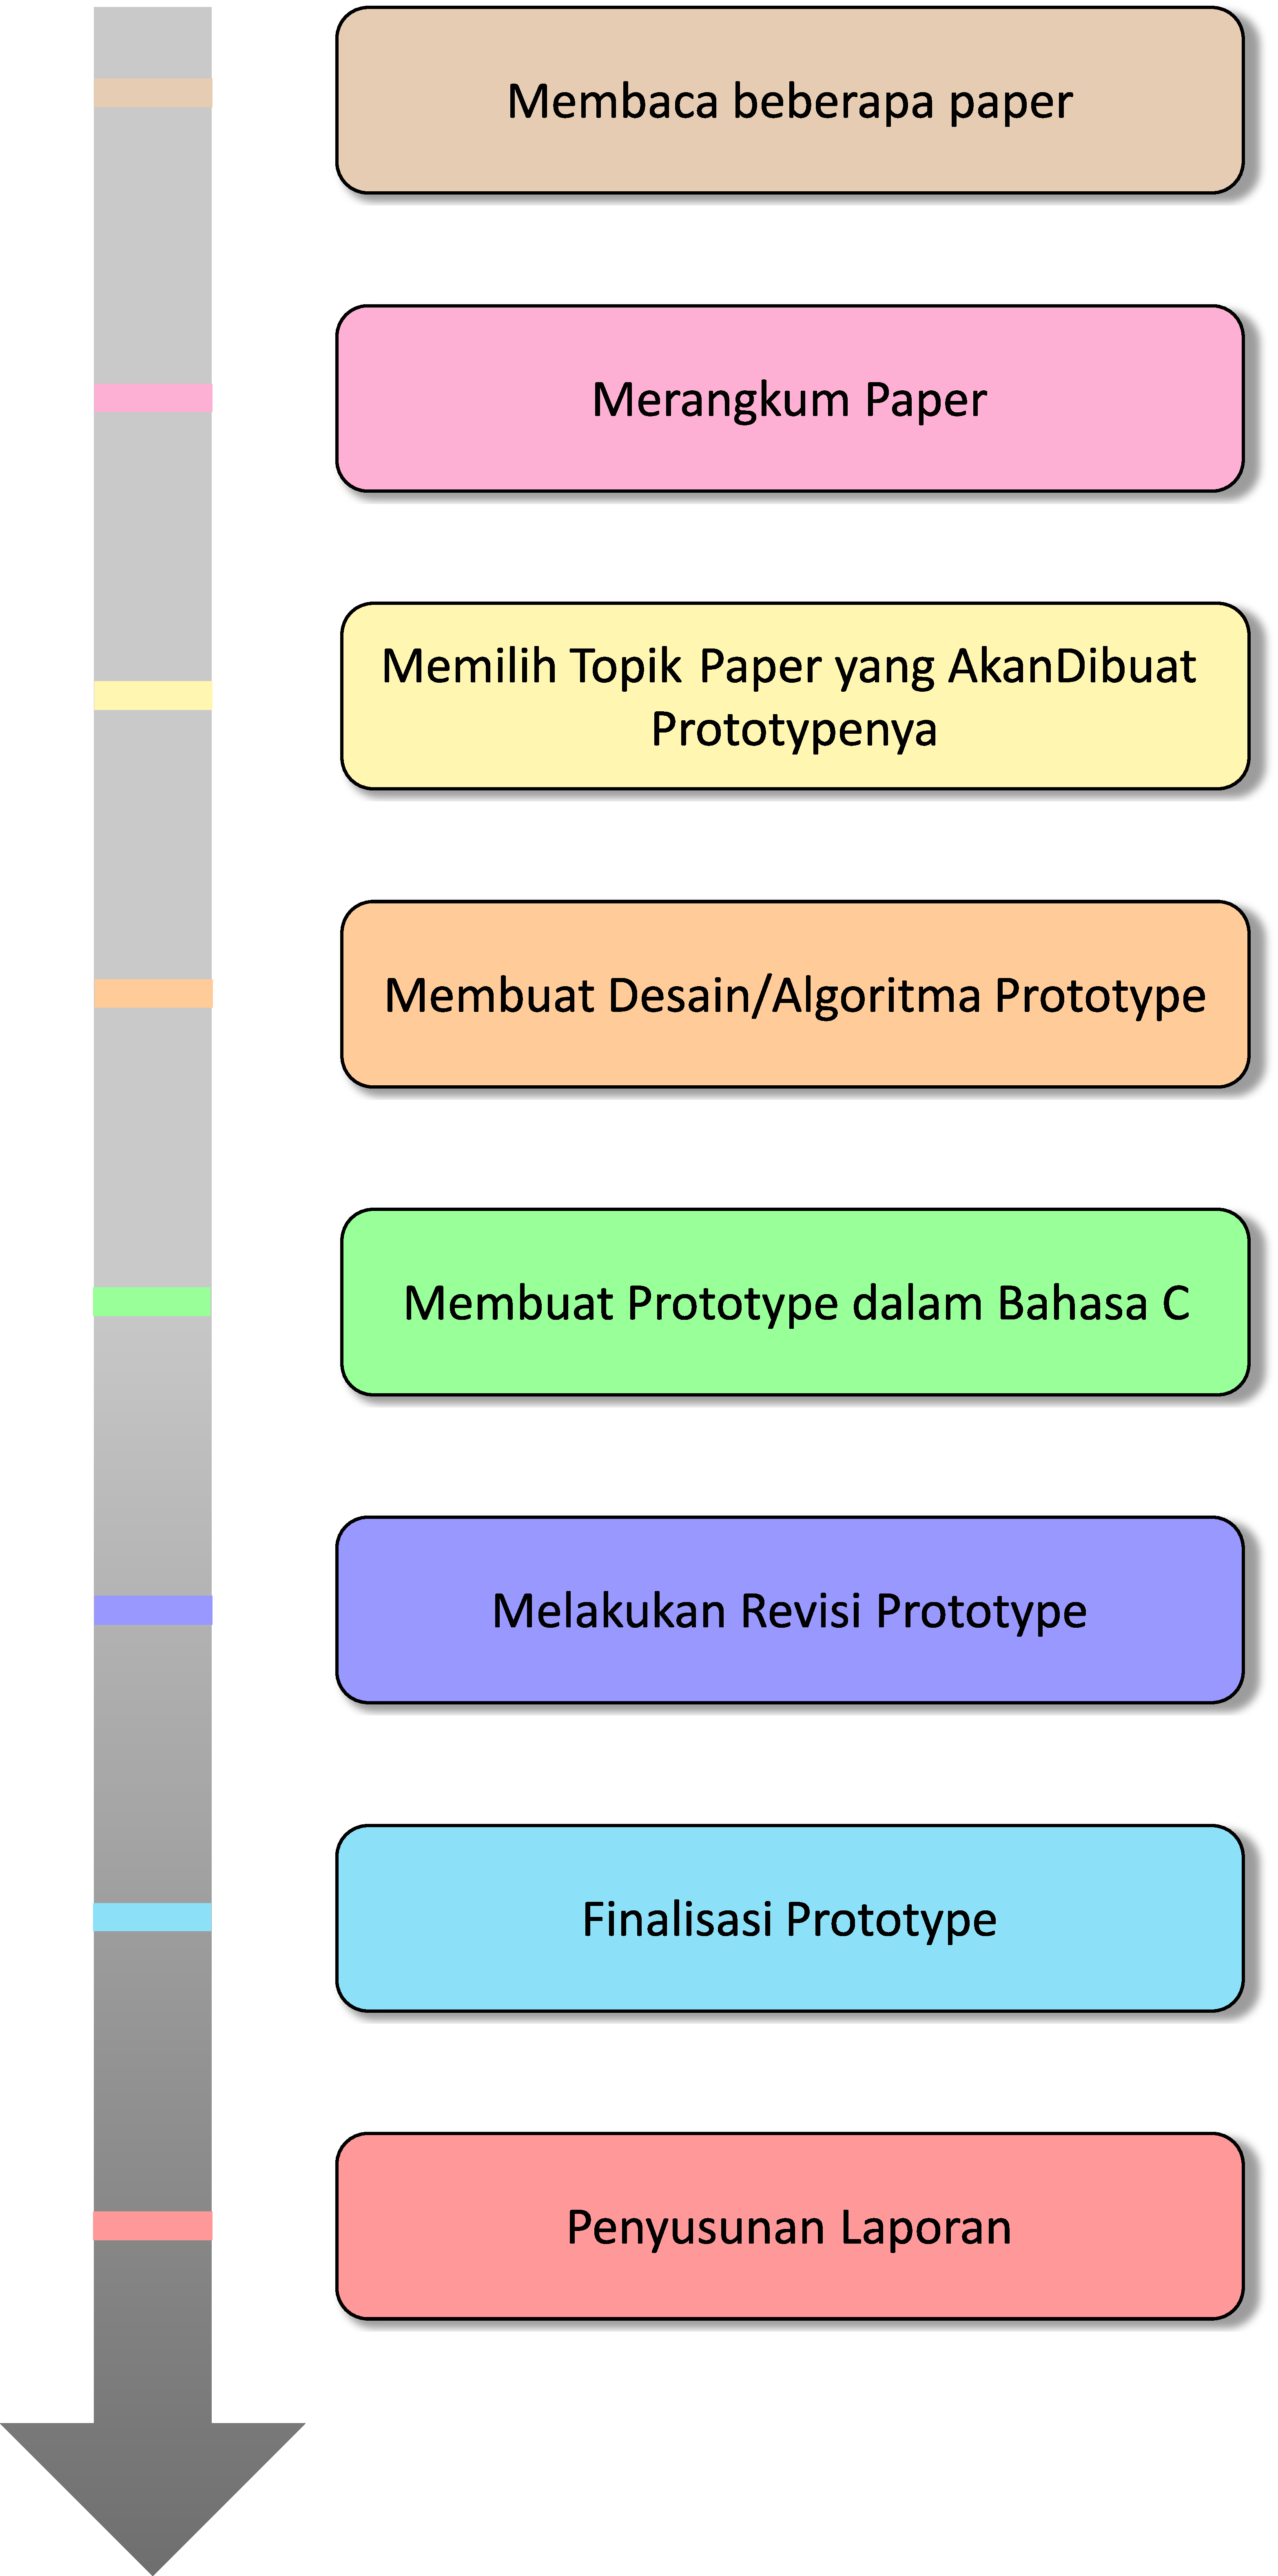
\includegraphics[width=0.4\textwidth]{gambar1}
\centering
\end{figure}


\section{Implemetasi dan Pegujian}
\subsection{Implementasi Graph pada Array dalam Bahasa C}
Program akan dimulai dengan pembacaan file bernama \textit{listtanaman.txt}. File tersebut akan menyimpan
informasi mengenai semua nama tanaman yang bersangkutan. Setelah pembacaan tersebut,
akan dicari informasi mengenai bobot graph yang menghubungkan \textit{node}. Informasi ini disimpandi dalam
matriks segitiga bawah kiri di dalam file \textit{jarakantarpohon.txt} yang juga dibuka saat program dijalankan.
Matriks menggambarkan bobot antara jarak dua \textit{node} tanaman sekali saja karena pemodelan \textit{undirected graph}
yang memiliki jarak sama baik dari $a$ ke $b$ maupun $b$ ke $a$. Nilai $-1$ akan menggambarkan bagian node yang tidak terhubung
sama sekali dalam graph dan juga dinyatakan dalam suatu variabel bernama int\_max(Jaraknya sebesar tak hingga). Nilai jarak terpendek
akan disimpan dalam array tersebut selagi program berjalan.

\subsection{Implementasi Algoritma Dijkstra dalam Bahasa C}
Dalam implementasi algoritma, abstraksi dengan menggunakan pseudocode dapat dibagi menjadi dua buah fungsi
dan satu program utama. Fungsi yang digunakan adalah fungsi printgraph (Fungsi Graph) untuk memunculkan graph
berukuran $n \times n$ ke layar pengguna. Algoritma dari fungsi tersebut dapat dilihat pada bagian di bawah ini:

\begin{algorithm}
\caption{Fungsi Graph \texttt{(printgraph)}}
\begin{algorithmic}
\State \textbf{Result:} Memunculkan Graph $n \times n$ Ke Layar
\State \textbf{procedure} \textit{printgraph(n, graph[n][n])}
\While{$ i \leq n-1$}
\State $j \leftarrow 0;$
\While{$ j \leq n-1$}
\If{$graph[i][j] - int\_max$}
\State{\textbf{output} ($-1$);}
\Else
\State{\textbf{output} ($graph[i][j]$);}
\EndIf
\State{$j \leftarrow j+1$;}
\EndWhile
\State{$i \leftarrow i+1$;}
\EndWhile
\end{algorithmic}
\end{algorithm}

Fungsi kedua yang digunakan adalah fungsi pencari indeks pada array yang akan diproses
dengan menggunakan pendekatan algoritma Dijkstra. Abstraksi fungsi yang digunakan dapat dilihat
pada bagian berikut ini:

\begin{algorithm}
\caption{Fungsi Pencari Indeks \texttt{(idx\_process)}}
\begin{algorithmic}
\State \textbf{Result:} Mencari indeks yang akan diproses dengan algoritma Dijkstra
\State \textbf{Initialization:}
\State \textit{$is\_found \leftarrow FALSE;$}
\State \textit{$i \leftarrow 0;$}
\State \textbf{Algoirthm:}
\While{$ i \leq n-1$}
\If{!$is\_final[i]$ \textbf{\textit{and}} !$is\_found$}
\State $idx\_min \leftarrow i$;
\State $val\_minimum \leftarrow jarak\_f[i]$;
\State $is\_found \leftarrow true$;
\EndIf
\If{$is\_found$ \textbf{\textit{and}} !$is\_final[i]$ \textbf{\textit{and}} $(jarak\_f[i] < val\_minimum)$}
\State $idx\_min \leftarrow i$;
\State $val\_minimum \leftarrow jarak\_f[i]$;
\EndIf
\EndWhile
\If{$is\_found$}
\State \textbf{return} ($idx\_min$)
\Else
\State \textbf{return} ($int\_max$)
\EndIf
\end{algorithmic}
\end{algorithm}

Program utama akan membaca file database tanaman beserta jarak masing-masing tanaman dan akan mencetak daftar
tanaman yang berada di Kebun Raya Purwodadi. Kemudian, program akan menerima input salah satu tanaman
terdekat dari pengguna sebagai penanda posisi awal pengguna. Setelah itu, program akan kembali menerima input
posisi tanaman tujuan dan memproses pencarian rute terdekat dengan algoritma Dijkstra. Rute yang diperlukan akan ditampilkan
dalam bentuk list nama tanaman yang harus dilalui pengguna dan menampilkan jarak antara kedua tanaman tersebut.
Implementasi algoritma dalam abstraksi tersebut dapat dilihat pada gambar di bawah ini:

\begin{algorithm}
\caption{Program Utama Pencarian Rute Antara Dua Tanaman - Pembacaan Jumlah Tanaman}
\begin{algorithmic}
\State \textbf{Result:} Menyimpan nama tanaman pada sebuah array
\State \textbf{Algorithm:}
\State \textbf{input}(\texttt{namafile\_tanaman});
\State \textbf{open}(\texttt{namafile\_tanaman});
\State \textbf{read}(\texttt{namafile\_tanaman});
\State \texttt{n\_tanaman} $\leftarrow$ \texttt{0};
\State \texttt{baris} $\leftarrow$ \texttt{0};
\While{\texttt{baris} $\leq$ \texttt{max\_len}}
\State \texttt{token} $\rightarrow$ \texttt{parse(baris)};
\State \texttt{token} $\rightarrow$ \texttt{nama\_tanaman[n\_tanaman]};
\State \texttt{n\_tanaman} $\rightarrow$ \texttt{n\_tanaman + 1};
\State \texttt{baris} $\rightarrow$ \texttt{baris+1};
\EndWhile
\end{algorithmic}
\end{algorithm}
Setelah pembacaan jumlah tanaman dari file, maka diperlukan graph atau jarak antar tanaman yang akan menjadi dasar
perhitungan dari pencarian rute terdekat. Proses memasukkan graph dapat dilihat pada algoritma berikut ini:
\begin{algorithm}
    \caption{Program Utama Pencarian Rute Antara Dua Tanaman - Memasukkan Graph}
    \begin{algorithmic}
    \State \textbf{Result:} Menyimpan graph dalam sebuah matriks $n \times n$
    \State \textbf{input}(\texttt{namafile\_graph});
    \State \textbf{open}(\texttt{namafile\_graph});
    \State \textbf{read}(\texttt{namafile\_graph});
    \State $baris \rightarrow 0$;
    \While{$baris \leq$ \texttt{max\_len}}
    \State $k \rightarrow 0$;
    \State $token \rightarrow parse(baris)$;
    \While{$ token! = NULL$}
    \State \texttt{graph[j][k]} $\rightarrow token$;
    \State \texttt{graph[k][j]} $\rightarrow token$;
    \If{$token == -1$}
    \State \texttt{graph[j][k]} $\rightarrow$ \texttt{int\_max}
    \State \texttt{graph[k][j]} $\rightarrow$ \texttt{int\_max}
    \Else
    \State $k \rightarrow k + 1$;
    \State $token \rightarrow parse(NULL)$;
    \EndIf
    \EndWhile
    \State $baris \rightarrow baris+1$;
    \EndWhile
    \end{algorithmic}
\end{algorithm}
Setelah data yang dibutuhkan dimasukkan, implementasi dari algoritma Dijkstra untuk pencarian
rute terdekat adalah sebagai berikut:

\begin{algorithm}
    \caption{Program Utama Pencarian Rute Antara Dua Tanaman: Pencarian Jarak dengan Algoritma Dijkstra}
    \begin{algorithmic}
    \State \textbf{Algorithm:}
    \State \textbf{input}(\texttt{idx\_a});
    \State \texttt{idx\_a} $\leftarrow$ \texttt{idx\_a-1};
    \State \textbf{input}(\texttt{idx\_tujuan});
    \State \texttt{idx\_tujuan} $\leftarrow$ \texttt{idx\_tujuan-1};
    \For{\textit{\texttt{i = 0} \textbf{to} \texttt{n\_tanaman}}}
    \If{\texttt{\textit{i = idx\_a}}}
    \State \texttt{jarak\_f[i]} $\leftarrow 0$;
    \State \texttt{is\_final[i]} $\leftarrow FALSE$;
    \Else
    \State \texttt{jarak\_f[i]} $\leftarrow$ \texttt{int\_max};
    \State \texttt{is\_final[i]} $\leftarrow FALSE$;
    \EndIf
    \For{\textit{\texttt{j = 0} \textbf{to} \texttt{n\_tanaman}}}
    \State \texttt{list\_dilalui[i][j]} $\leftarrow$ \texttt{int\_max};
    \EndFor
    \State \texttt{idx\_lalui[i]} $\leftarrow 0$;
    \EndFor
    \State \texttt{jarak\_f[idx\_a]} $\leftarrow 0$;
    \State \texttt{list\_dilalui[idx\_a][0]} $\leftarrow$ \texttt{idx\_a};
    \State \texttt{idx\_lalui[idx\_a]} $\leftarrow$ \texttt{idx\_lalui[idx\_a]+1};
    \State \texttt{idx\_now} $\leftarrow$ \texttt{idx\_a};
    \While{\textit{\texttt{idx\_now! = int\_max}}}
    \State \texttt{is\_final[idx\_now]} $\leftarrow TRUE$;
    \For{\textit{\texttt{i = 0} \textbf{to} \texttt{n\_tanaman-1}}}
    \If{\textit{\texttt{!is\_final[i]} \textbf{and} \texttt{graph[idx\_now][i]! = int\_max} \textbf{and} \texttt{(jarak\_f[idx\_now] + graph[idx\_now][i]) > jarak\_f[i]}}}
    \State \texttt{jarak\_fi]} $\leftarrow$ \texttt{(jarak\_f[idx\_now] + graph[idx\_now][i])};
    \State \texttt{idx\_lalui[i]} $\leftarrow$ \texttt{idx\_lalui[idx\_now] + 1};
    \EndIf
    \For{\textit{\texttt{j=0} \textbf{to} \texttt{idx\_dilalui[i]-1}}}
    \If{\textit{\texttt{j=idx\_dilalui[i]-1}}}
    \State \texttt{list\_dilalui[i][j]} $\leftarrow$ \texttt{i};
    \Else
    \State \texttt{list\_dilalui[i][j]} $\leftarrow$ \texttt{list\_dilalui[idx\_now][j]};
    \EndIf
    \EndFor
    \EndFor
    \State \texttt{idx\_now} $\leftarrow$ \texttt{idx\_process(n\_tanaman, jarak\_f, is\_final)};
    \EndWhile
    \end{algorithmic}
\end{algorithm}

\subsection{Perhitungan Kompleksitas Waktu}
Kompleksitas dari program ini dengan notasi kompleksitas Big O adalah $O(n^2)$. Hal tersebut disebabkan pada loop program
bagian \textit{for}, terdapat loop \textit{for} lain yang berjumlah dua loop (Terletak pada bagian \textit{assign} kondisi awal
dan ketika program menjalankan algoritma Dijkstra). Karena hal tersebut, akibatnya adalah kompleksitas waktu akan naik seiring dengan
naiknya $n$ program yang dijalankan, namun tidak bersifat linear sehingga kompleksitas waktunya adalah $O(n^2)$. Grafik kompleksitas waktu dapat
direpresentasikan pada gambar 1. 
\begin{figure}[htbp]
    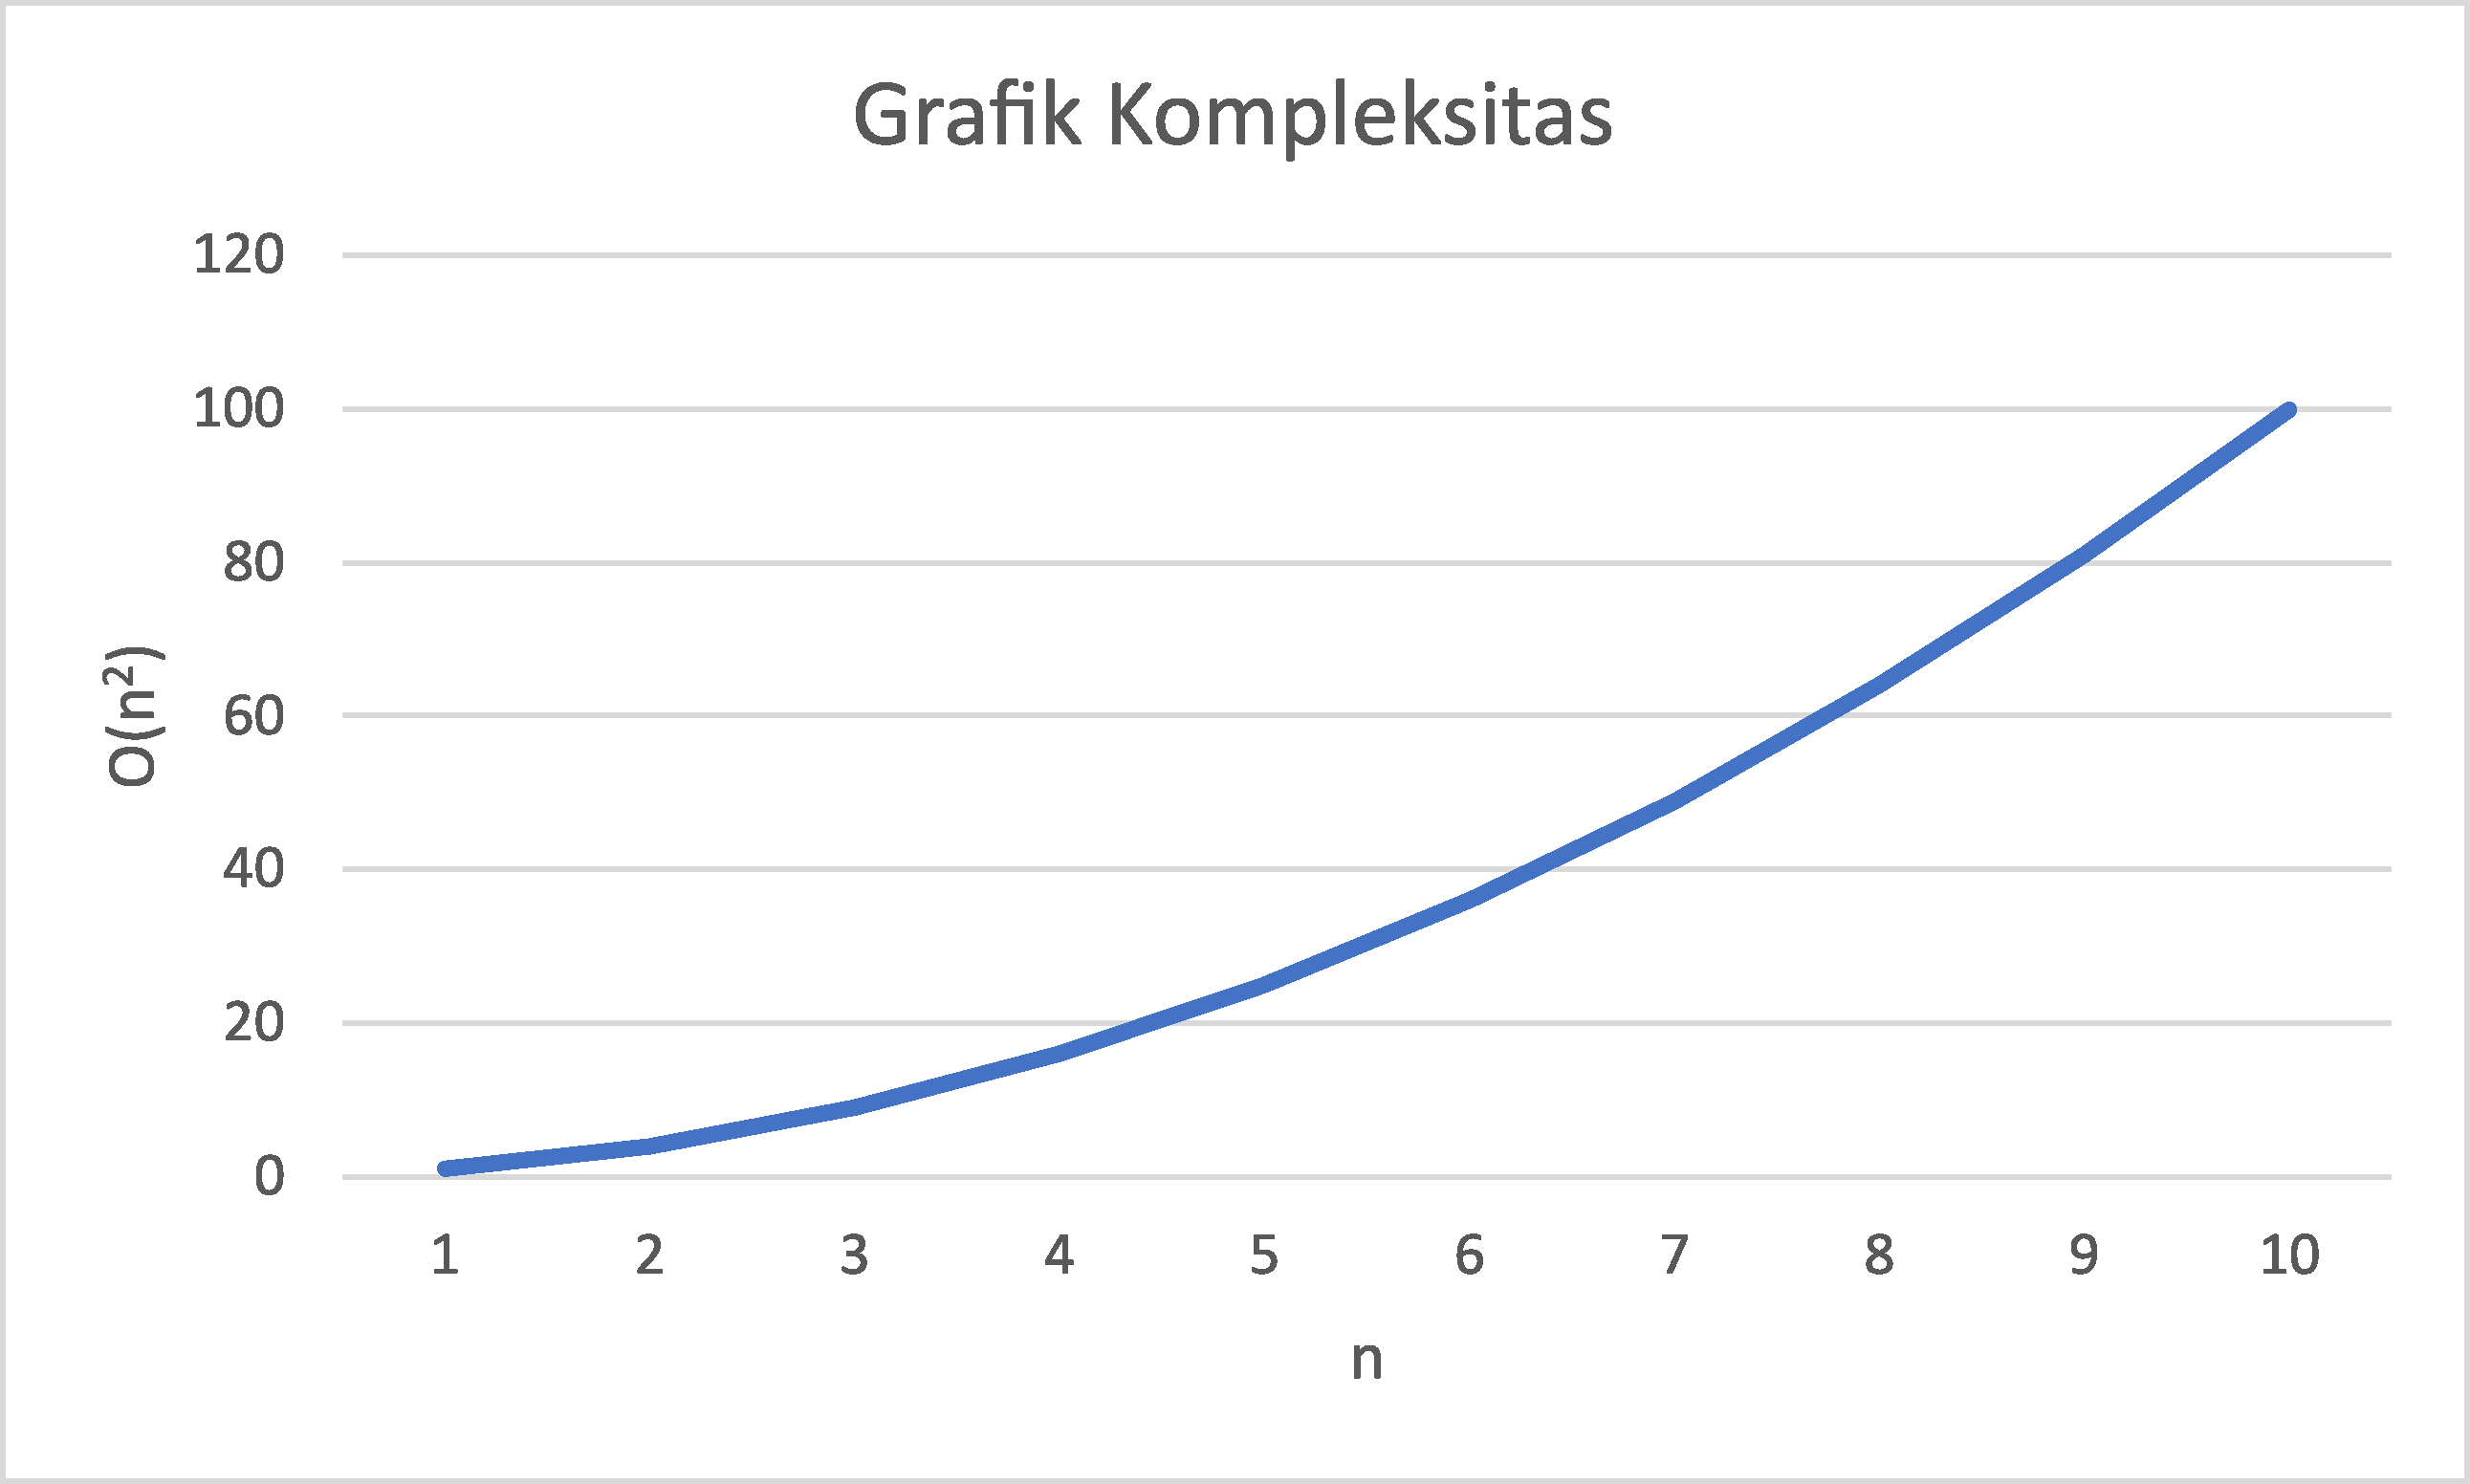
\includegraphics[width=0.4\textwidth]{kompleksitas}
    \centering
    \caption{Kompleksitas Waktu Program}
    \label{fig:mesh1}
\end{figure}

\subsection{Perhitungan Kompleksitas Tempat}
Matriks penyimpanan yang digunakan pada program ini memiliki ukuran terbesar $n \times n$, dengan nilai
$n$ merepresentasikan banyak tanaman dalam file \textit{listtanaman.txt}. Program akan melalui grafik dan menyimpan
nilai bobot antara \textit{node} sebesar matriks di atas, mengakibatkan program dengan kompleksitas $O(n^2)$. Hal ini dapat
dilihat pada grafik kompleksitas tempat di gambar 2.
\begin{figure}[htbp]
    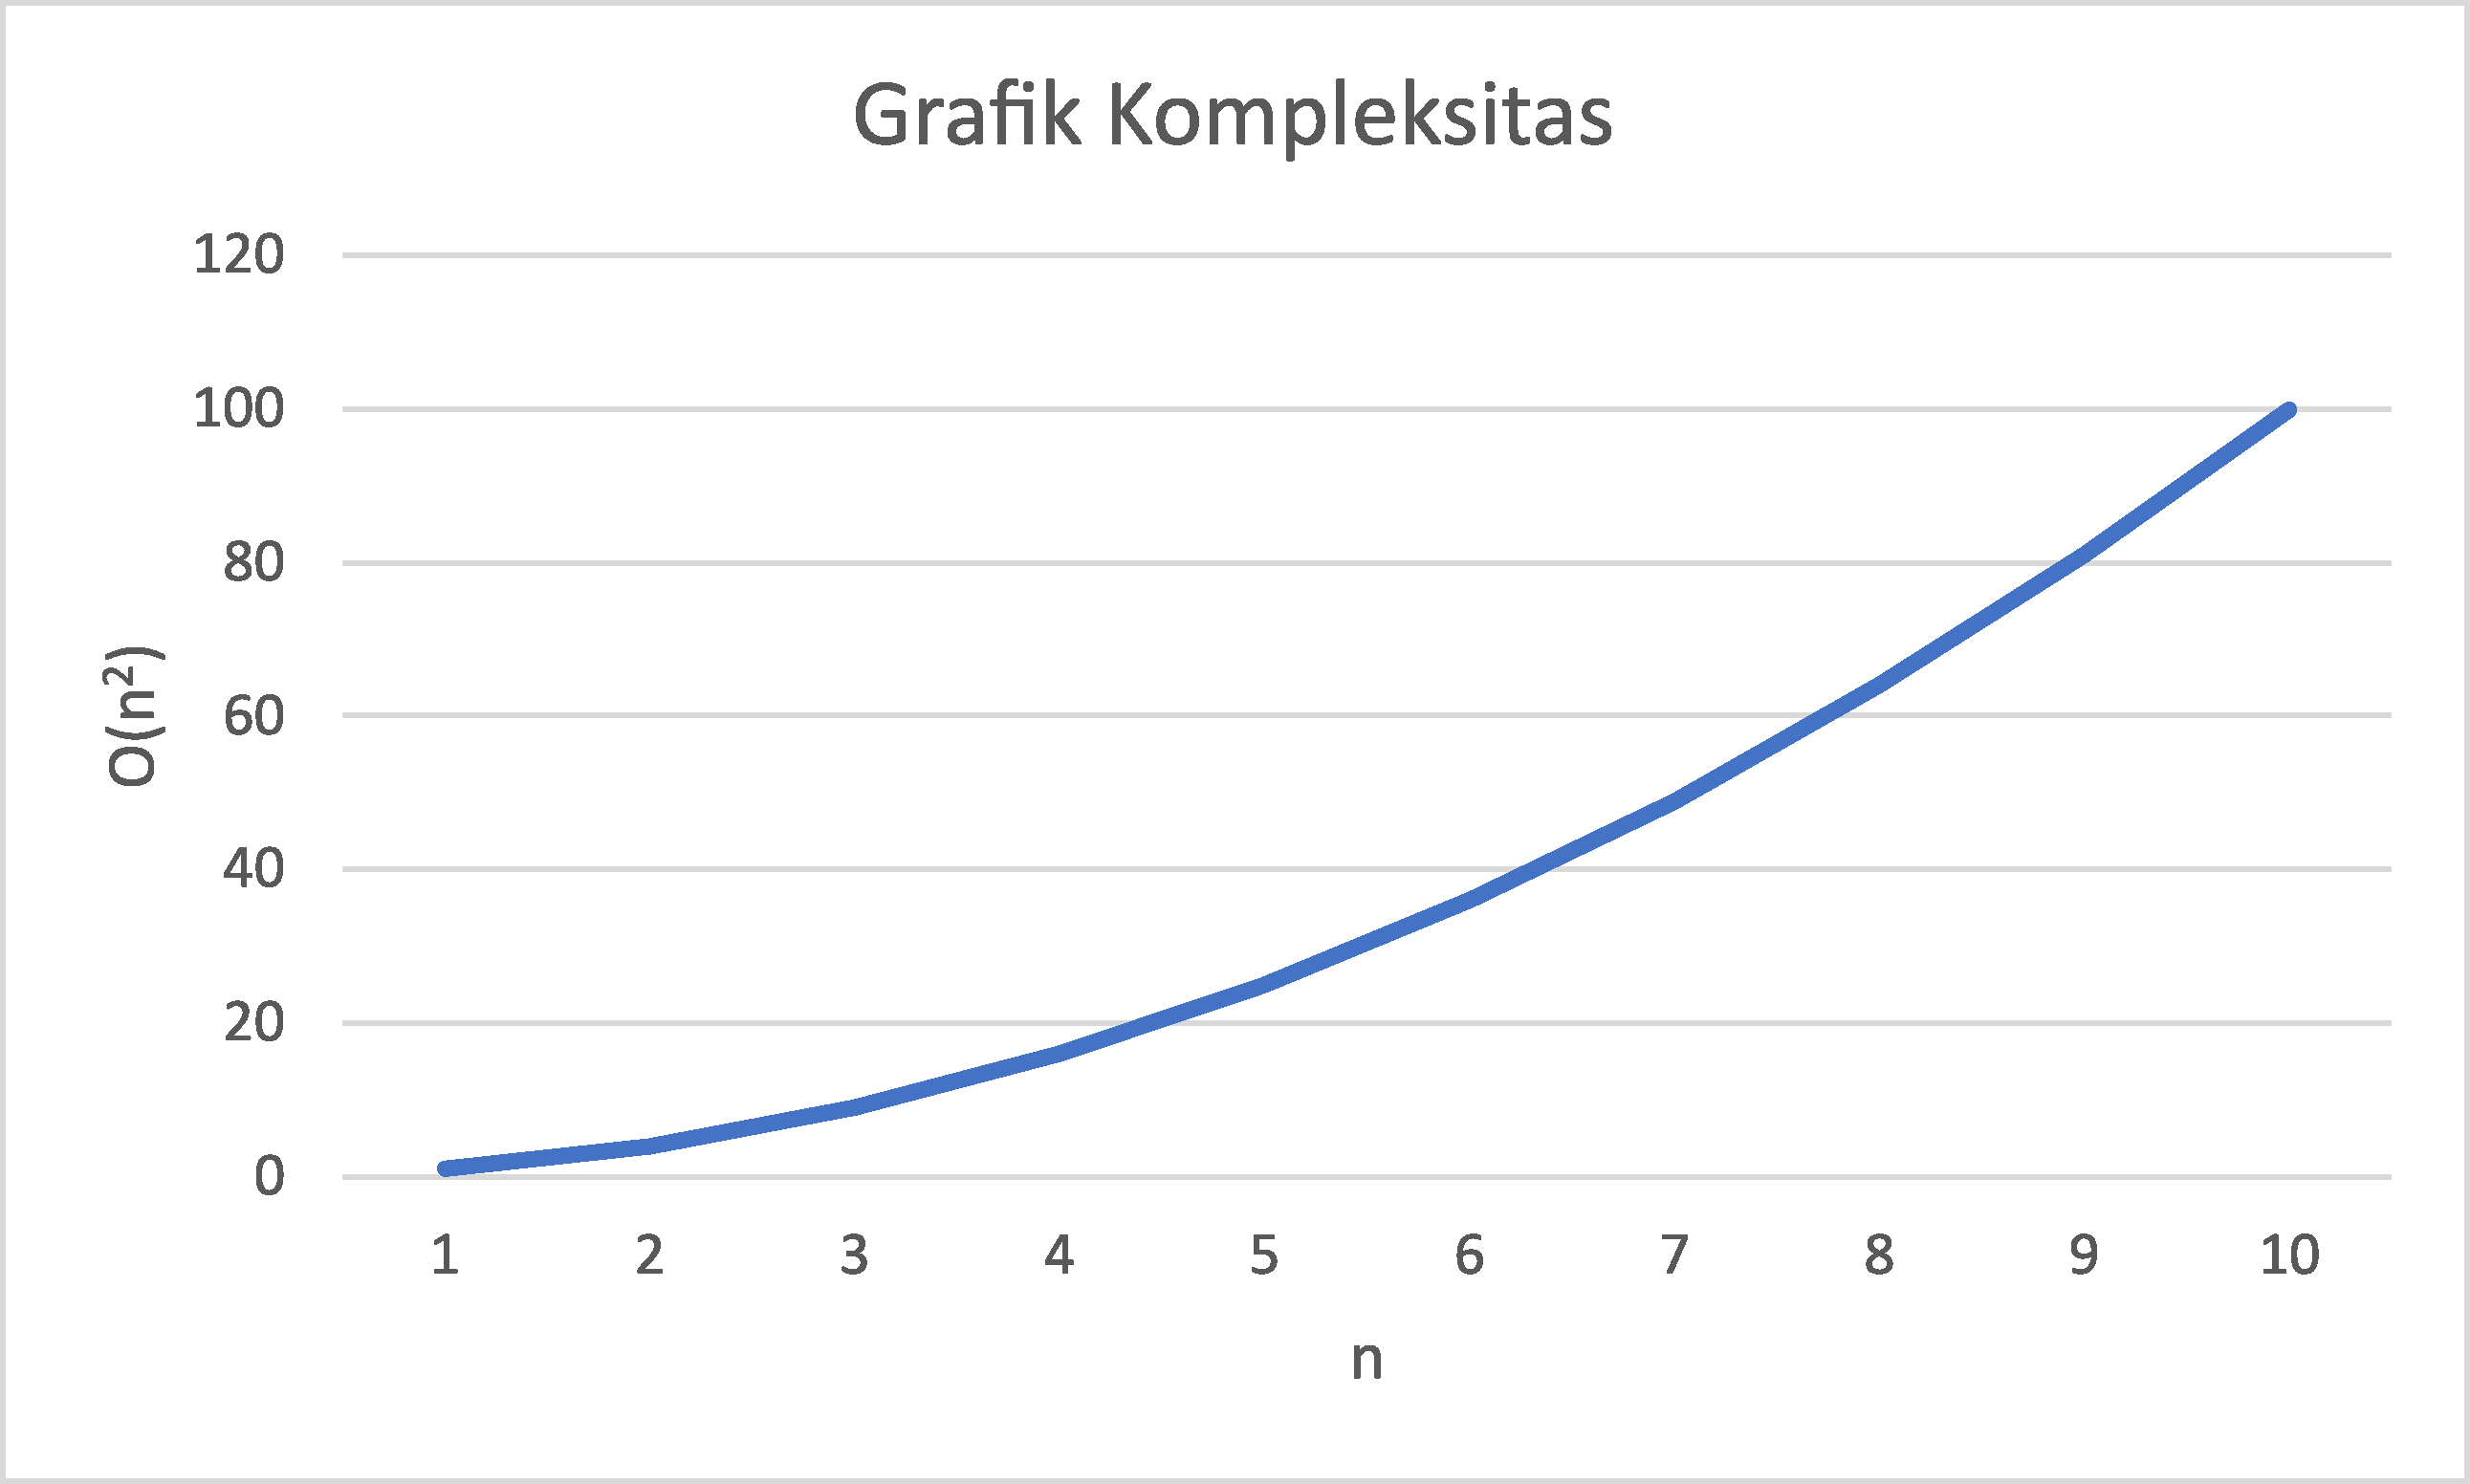
\includegraphics[width=0.4\textwidth]{kompleksitas}
    \centering
    \caption{Kompleksitas Tempat Program}
    \label{fig:mesh2}
\end{figure}


\section{Kesimpulan}
Pada perhitungan Jarak Terdekat dalam suatu lokasi atau ruang dapat diimplementasikan penggunaan Algoritma Dijkstra
dalam perhitungannya untuk mencapai suatu target pada ruang tersebut dari suatu titik. Terbukti dari penilitian
Kebun Raya Purwodadi untuk menentukan Tanaman yang ingin dituju.


\bibliographystyle{IEEEtran}
\bibliography{references.bib}
\end{document}
